\chapter{الحياة عبر فصول السنة}\label{ch:g6:life-through-seasons}

صوّر شجرة الكستناء نفسها في أول كل شهر وثبّت الصور الاثنتي عشرة في
صف: \omterm{def:g1:plants-around-us:tree}{أغصان} عارية، \omterm{def:g6:life-through-seasons:buds}{فبراعم}، \omterm{def:g1:plants-around-us:parts}{فأوراق}، فشمعات من الأزهار، \omterm{prop:g3:flowers-fruits-seeds:transform}{فثمار}، فذهب،
\omterm{def:g1:plants-around-us:tree}{فأغصان} عارية من جديد. لم يتحرك شيء --- فالشجرة وقفت ساكنة السنة
كلها --- ومع ذلك تغير كل شيء. وقد تتبع
\cref{ch:g3:animals-through-seasons} \omterm{def:g1:animals-around-us:animal}{الحيوانات} عبر السنة؛ والآن،
بعينَي ماسح، نتتبع \omterm{def:g6:exploring-our-environment:components}{البيئة} كلها، \omterm{def:g1:plants-around-us:plant}{والنباتات} أولًا.

\section{البيئة تتغير مع فصول السنة}

\begin{proposition}[التغير الموسمي في الشروط]\label{prop:g6:life-through-seasons:conditions}
عبر السنة تتأرجح \omterm{def:g6:exploring-our-environment:conditions}{شروط} \omterm{def:g6:exploring-our-environment:components}{البيئة}
(\cref{def:g6:exploring-our-environment:conditions}) تأرجحًا
واسعًا: فالأيام تقصر وتطول، والحرارات تهبط وترتفع، وندى التربة
يتبع المطر والجفاف. والموقع الممسوح في كانون الثاني وفي حزيران
يعطي سطرين مختلفين في الجدول --- ومن ثم، وفق
\cref{prop:g6:exploring-our-environment:decide}، توقّع طاقمين
مختلفين من السكان.
\end{proposition}
\admitted

\begin{example}[سياج واحد ومسحان]\label{ex:g6:life-through-seasons:hedge}
سياج الممر، ممسوحًا مرتين. حزيران: \omterm{def:g1:plants-around-us:parts}{أوراق} كثيفة، وعشرة \omterm{def:g5:biodiversity:species}{أنواع} نباتية
مزهرة عند قدمه، ونحل يضجّ، وشحارير تعشّش، وحلزونات بعد المطر.
وكانون الثاني: \omterm{def:g1:plants-around-us:tree}{أغصان} عارية، والأخضر مختزل في اللبلاب والطحلب، ولا
حشرة تطير، وشحارير تنقّب في فرش \omterm{def:g1:plants-around-us:parts}{الأوراق}، وحلزونات مختومة في
أصدافها في عمق الضفة. المكان نفسه، وقائمة المكوّنات نفسها ---
حي، ومعدني، وآثار --- لكن عمود الحي قد تحوّل.
\end{example}

\section{كيف تعبر النباتات الموسم الصعب}

\begin{definition}[النفضية ودائمة الخضرة]\label{def:g6:life-through-seasons:trees}
تنقسم الأشجار بحسب جوابها عن الشتاء:
\begin{itemize}
  \item الأشجار \emph{النفضية}\index{نفضي} --- كالبلوط
        والكستناء والزان --- تُسقط أوراقها كلها في الخريف وتقف
        عارية؛
  \item والأشجار \emph{دائمة الخضرة}\index{دائم الخضرة} ---
        كالصنوبر والبهشية واللبلاب على الجدار --- تُبقي أوراقًا
        عاملة طول الشتاء، وهي في العادة قاسية أو شمعية أو إبرية
        (وقد لقيت \cref{prop:g3:sorting-living-things:plants}
        الإبر من قبل).
\end{itemize}
\end{definition}

\begin{definition}[البراعم]\label{def:g6:life-through-seasons:buds}
الشجرة \omterm{def:g6:life-through-seasons:trees}{النفضية} في الشتاء ليست ميتة: فربيعها القادم محزوم على
أغصانها منذ الآن \emph{براعم}\index{برعم} --- وهي أفرخ كاملة
صغيرة، أوراقها مطوية في حجم صغير، ملفوفة في حراشف تصدّ الطقس.
\omterm{def:g1:plants-around-us:parts}{فأوراق} الربيع ``الجديدة'' بُنيت في الصيف السابق؛ والبرعم مخزنها
الشتوي.
\end{definition}

\begin{example}[فتح برعم كستناء الحصان]\label{ex:g6:life-through-seasons:bud}
\omterm{def:g6:life-through-seasons:buds}{براعم} كستناء الحصان الكبيرة اللزجة تنفتح جيدًا تحت نصل (وهو عمل
يقوم به كبير): فتحت الحراشف المطلية، محزومة في زغب قطني، تقع
\omterm{def:g1:plants-around-us:parts}{أوراق} صغيرة مطوية --- تامة، شاحبة، منتظرة. \omterm{def:g1:plants-around-us:tree}{والغصن} المقطوع في شباط
الموضوع في ماء داخل البيت ``يورق'' قبل موعده بأسابيع: فالأفرخ
كانت جاهزة؛ ولم يكن ينقصها إلا الدفء.
\end{example}

\begin{omfigure}
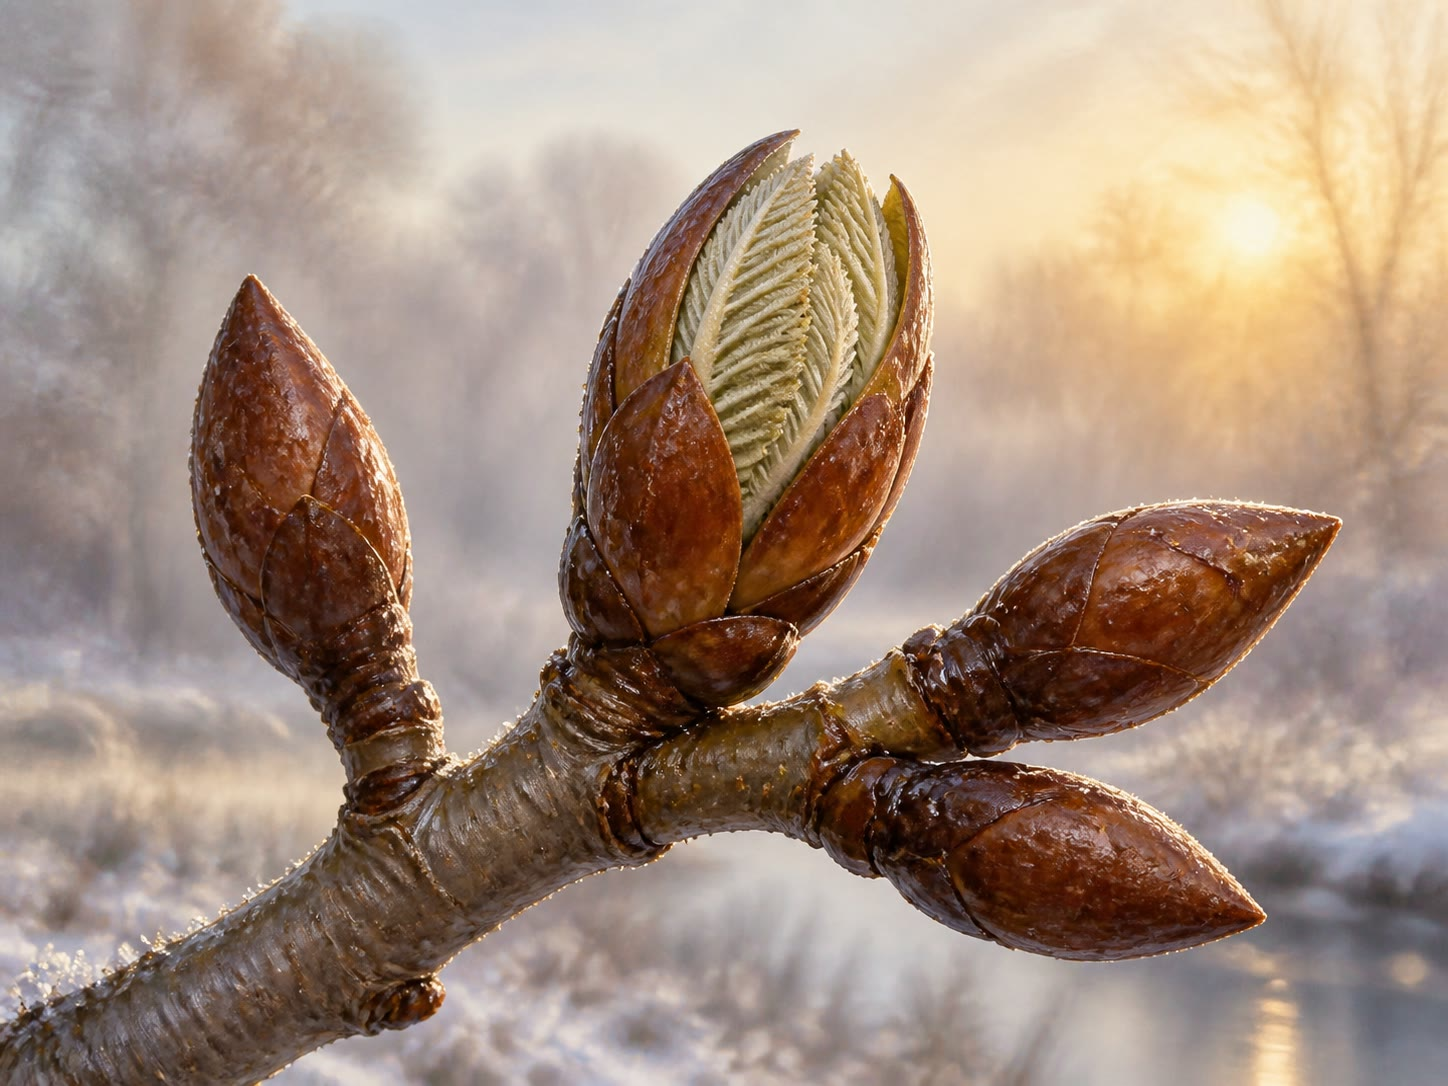
\includegraphics[width=0.56\linewidth]{images/book1/ai/g6-seasons-buds.jpg}

{\small المخزن الشتوي مفتوحًا: داخل حراشف \omterm{def:g6:life-through-seasons:buds}{برعم} كستناء الحصان
المطلية تقع \omterm{def:g1:plants-around-us:parts}{أوراق} الربيع القادم مطوية جاهزة.}
\end{omfigure}

\begin{proposition}[أجوبة الطبقة العشبية عن الشتاء]\label{prop:g6:life-through-seasons:herbs}
وللنباتات الأصغر خططها الخاصة:
\begin{itemize}
  \item \emph{النباتات الحولية}\index{نبات حولي} --- كالخشخاش
        والفول --- تموت كلها في الخريف وتعبر الشتاء
        \emph{بذورًا} (\cref{prop:g2:from-seed-to-plant:needs}:
        \omterm{def:g2:from-seed-to-plant:seed}{فالبذرة} تنتظر البرد بأمان)؛
  \item و\emph{النباتات المعمَّرة}\index{نبات معمَّر} ---
        كالنرجس والهندباء --- تدع أعاليها تموت وتنتظر تحت الأرض
        أبصالًا أو \omterm{ex:g4:plants-without-seeds:bulbtuber}{درنات} أو أصولًا قاسية
        (وهي مخازن \cref{ex:g4:plants-without-seeds:bulbtuber}
        تؤدي خدمة الشتاء)؛
  \item ودائمات الخضرة الأرضية --- كالطحلب واللبلاب --- تصبر
        ببساطة.
\end{itemize}
\end{proposition}
\admitted

\begin{example}[أين ذهب النرجس؟]\label{ex:g6:life-through-seasons:daffodil}
رقعة النرجس تزهر في آذار، وتصفرّ في أيار، وفي تموز تكون قد اختفت
بلا أثر --- ومع ذلك تعود في آذار التالي أكثف. فقد كانت طول الصيف
والخريف والشتاء أبصالًا تحت العشب: \omterm{def:g1:plants-around-us:plant}{فالنبات} لم يرحل؛ بل انسحب إلى
المخزن.
\end{example}

\section{تقويم الحيوانات من جديد}

\begin{proposition}[أجوبة الحيوانات بلغة المسح]\label{prop:g6:life-through-seasons:animals}
خطط \cref{ch:g3:animals-through-seasons} الثلاث --- \omterm{def:g3:animals-through-seasons:migration}{الهجرة}،
\omterm{def:g3:animals-through-seasons:hibernation}{والسبات}، والبقاء نشطًا --- تُقرأ الآن أجوبةً عن التغيرات الممسوحة:
فكل \omterm{def:g5:biodiversity:species}{نوع} يتعقب شروطه وغذاءه اللذين يحتاج إليهما.
\begin{itemize}
  \item السنونو يتبع مورد غذائه إلى حيث تُبقي \omterm{def:g6:exploring-our-environment:conditions}{الشروط} \omterm{prop:g3:sorting-living-things:groups}{الحشرات}
        طائرة؛
  \item والقنفذ والحلزون المختوم ينتظران الشهور التي لا تستطيع
        أجسامهما العمل خلالها؛
  \item \omterm{prop:g3:sorting-living-things:groups}{والحشرات} تضيف جوابًا رابعًا: فأكثرها يعبر الشتاء
        \emph{بيضًا أو \omterm{ex:g2:animals-grow-up:butterfly}{يرقات} أو شرانق}
        (\cref{ex:g2:animals-grow-up:butterfly}) مدسوسة في
        التربة أو اللحاء أو فرش \omterm{def:g1:plants-around-us:parts}{الأوراق} --- فيموت البالغ، ويشتّي
        \omterm{def:g5:biodiversity:species}{النوع} في مراحله الصغيرة.
\end{itemize}
\end{proposition}
\admitted

\begin{example}[أين حشرات حزيران في كانون الثاني]\label{ex:g6:life-through-seasons:insects}
سياج كانون الثاني لا يُظهر حشرة --- ومع ذلك فحشرات حزيران كلها
حاضرة: الفراشات شرانق تحت حجارة القمة، والجنادب بيضًا في التربة،
والدعسوقات بالغات نائمات متجمعات في عمق فرش \omterm{def:g1:plants-around-us:parts}{الأوراق}، والنحل
عنقودًا دافئًا متراصًّا في \omterm{def:g5:first-look-at-cells:cell}{الخلية}. فمسح حزيران يمشي؛ أما مسح كانون
الثاني فعليه أن يحفر ويرفع ويحدّق --- فالسكان غيّروا \emph{صورتهم}
لا عنوانهم.
\end{example}

\begin{method}[المسح عبر السنة]\label{met:g6:life-through-seasons:yearsurvey}
لتدرس حياة موقع عبر المواسم:
\begin{enumerate}
  \item امسح الموقع المعلَّم نفسه
        (\cref{met:g6:exploring-our-environment:survey}) مرة في
        كل موسم --- المربع نفسه، والأدوات نفسها، وزمن التفتيش
        نفسه؛
  \item وسجّل \omterm{def:g6:exploring-our-environment:conditions}{الشروط} \emph{والسكان} في كل مرة؛ وصوّر الموقع من
        البقعة نفسها؛
  \item وفتّش عن صور الشتاء المختفية عن قصد: \omterm{def:g6:life-through-seasons:buds}{البراعم}، والأبصال،
        \omterm{def:g2:animals-grow-up:born}{والبيض}، والشرانق، والحلزونات المختومة --- وأعد كل غطاء
        إلى مكانه؛
  \item وضع المسوح الأربعة جنبًا إلى جنب: واقرن كل تغير في
        السكان بتغير في \omterm{def:g6:exploring-our-environment:conditions}{الشروط}، وسمِّ صورة كل غائب الشتوية أو
        وجهته.
\end{enumerate}
\end{method}

\begin{remark}[لا شيء يختفي ببساطة]\label{rem:g6:life-through-seasons:vanish}
يعلّمنا جدول السنة كلها قاعدة عميقة واحدة: لا نوع من \omterm{def:g5:biodiversity:species}{أنواع} مسح
حزيران قد زال ببساطة. فكل واحد إما في مكان آخر (مهاجرًا)، أو نائم
(سابتًا)، أو في المخزن (\omterm{ex:g4:plants-without-seeds:bulbtuber}{بصلة} أو \omterm{def:g2:from-seed-to-plant:seed}{بذرة})، أو في مرحلة حياة أخرى (\omterm{def:g2:animals-grow-up:born}{بيضة}
أو شرنقة). وكلمة ``ذهب'' ليست جوابًا كاملًا في \omterm{def:g1:living-or-not:living}{علم الأحياء} --- والسؤال
التالي دائمًا: \emph{ذهب إلى أين، وبأي صورة؟}
\end{remark}

\section{تمارين}

\begin{exercise}[$\star$]\label{exo:g6:life-through-seasons:1}
أي \omterm{def:g6:exploring-our-environment:conditions}{شروط} الموقع تتأرجح مع المواسم؟ سمِّ ثلاثة.
\end{exercise}

\begin{exercise}[$\star$]\label{exo:g6:life-through-seasons:2}
\omterm{def:g6:life-through-seasons:trees}{نفضي} أم \omterm{def:g6:life-through-seasons:trees}{دائم الخضرة}: البلوط، والصنوبر، والزان، والبهشية، وكستناء
الحصان؟ وما معنى كل كلمة؟
\end{exercise}

\begin{exercise}[$\star$]\label{exo:g6:life-through-seasons:3}
ما الذي في داخل \omterm{def:g6:life-through-seasons:buds}{البرعم} الشتوي، ومتى بُني؟
\end{exercise}

\begin{exercise}[$\star$]\label{exo:g6:life-through-seasons:4}
كيف يعبر \omterm{prop:g6:life-through-seasons:herbs}{النبات الحولي} الشتاء؟ وكيف يعبره معمَّر كالنرجس؟
\end{exercise}

\begin{exercise}[$\star$]\label{exo:g6:life-through-seasons:5}
اشرح \omterm{def:g1:plants-around-us:tree}{غصن} شباط في \cref{ex:g6:life-through-seasons:bud}: لماذا
يستطيع أن يورق قبل موعده بأسابيع داخل البيت؟
\end{exercise}

\begin{exercise}[$\star$]\label{exo:g6:life-through-seasons:6}
أعطِ أجوبة \omterm{def:g1:animals-around-us:animal}{الحيوانات} الأربعة عن الشتاء، مع \omterm{def:g5:biodiversity:species}{نوع} واحد لكل جواب.
\end{exercise}

\begin{exercise}[$\star\star$]\label{exo:g6:life-through-seasons:7}
لكل ساكن من سكان سياج حزيران، سمِّ صورته وعنوانه في كانون الثاني:
الفراشة، والجندب، والدعسوقة، والحلزون، والسنونو.
\end{exercise}

\begin{exercise}[$\star\star$]\label{exo:g6:life-through-seasons:8}
لماذا يجب أن تستعمل المسوح الموسمية الأربعة الموقع نفسه والأدوات
نفسها وزمن التفتيش نفسه؟ وأي قاعدة من
\cref{ch:g6:exploring-our-environment} تعمل هنا؟
\end{exercise}

\begin{exercise}[$\star\star$]\label{exo:g6:life-through-seasons:9}
مسح سياج كانون الثاني يعدّد كائنات حية أقل بكثير من مسح حزيران.
أعطِ سببين يجعلان الفرق يبالغ في الفقد الحقيقي، مستعملًا
\cref{ex:g6:life-through-seasons:insects}.
\end{exercise}

\begin{exercise}[$\star\star$]\label{exo:g6:life-through-seasons:10}
يحفر بستاني أرض نرجس ``ميتة'' في آب فيجد أبصالًا متينة. ترجم ما
وجده وفق \cref{prop:g6:life-through-seasons:herbs}: في أي حال
\omterm{def:g1:plants-around-us:plant}{النبات}، وماذا ستفعل الأبصال في آذار؟
\end{exercise}

\begin{exercise}[$\star\star$]\label{exo:g6:life-through-seasons:11}
طبّق \cref{rem:g6:life-through-seasons:vanish}: ضفادع بركة لا
تُوجد البتة في كانون الثاني. أعطِ السؤالين اللذين يُسألان، وجواب
الضفادع والعلاجيم عنهما.
\end{exercise}

\begin{exercise}[$\star\star\star$]\label{exo:g6:life-through-seasons:12}
\omterm{def:g1:plants-around-us:parts}{أوراق} دائمات الخضرة قاسية أو شمعية أو إبرية؛ \omterm{def:g1:plants-around-us:parts}{وأوراق} النفضيات
عريضة رقيقة. اقترح أي مشكلة من مشكلات الشتاء تجيب عنها بنية \omterm{def:g1:plants-around-us:parts}{ورقة}
\omterm{def:g6:life-through-seasons:trees}{دائمة الخضرة} (فكّر في متاعب ماء حشرة القمل الخشبي معكوسة)، ولماذا
تفضّل الشجرة \omterm{def:g6:life-through-seasons:trees}{النفضية} أن تُسقط أوراقها الرقيقة بدل ذلك.
\end{exercise}

\section{مسألة: الصور الاثنتا عشرة}

\begin{problem}[{مسألة نهاية الأسبوع --- سنة من حياة شجرة
الكستناء، مقروءةً صورةً صورة}]\label{pb:g6:life-through-seasons:1}
تصوّر لينا شجرة الكستناء عند البوابة في أول كل شهر مدة سنة، وتثبّت
الصور الاثنتي عشرة في صف. وتكتب تحت كل صورة طول النهار وحرارة
الصباح.

\medskip\noindent\textbf{القسم الأول --- قراءة الصف.}
\begin{enumerate}
  \item تُظهر صورتا كانون الثاني وكانون الأول أغصانًا عارية. فما
        الذي على \omterm{def:g1:plants-around-us:tree}{الأغصان} يثبت أن الشجرة حية ومستعدة للربيع في
        الصورتين؟
  \item بين أي صورتين تنفتح \omterm{def:g6:life-through-seasons:buds}{البراعم}؟ وملاحظات لينا هناك تقول:
        النهار $11$--$13$ ساعة، والصباح
        $8$--\qty{12}{\degreeCelsius}. فأي \omterm{def:g6:exploring-our-environment:conditions}{الشروط} المتغيرة
        تجيب عنها الشجرة؟
  \item تُظهر صورة أيار ``شمعات'' منتصبة من الأزهار البيضاء.
        مستعملًا \cref{ch:g3:flowers-fruits-seeds} (أو
        \cref{ch:g5:flower-to-fruit})، ما الذي يجب أن يزور بين
        صورتي أيار وأيلول لتوجد \omterm{prop:g3:flowers-fruits-seeds:transform}{ثمار} تشرين الأول --- وما \omterm{prop:g3:flowers-fruits-seeds:transform}{الثمرة}
        بالضبط؟
  \item تُظهر صورة تشرين الأول أوراقًا ذهبية؛ وتُظهر صورة تشرين
        الثاني أغصانًا عارية وفرشًا بنيًّا تحتها. سمِّ صنف الشجرة
        من \cref{def:g6:life-through-seasons:trees}، وأين
        يُخزَّن ربيعها القادم عبر الصور التالية.
\end{enumerate}

\medskip\noindent\textbf{القسم الثاني --- جيران الشجرة.}
\begin{enumerate}[resume]
  \item تحت الشجرة تلتقط صورة آذار رقعة نرجس غائبة عن صورة تموز.
        فأين الرقعة في تموز، وبأي صورة؟
  \item يحفّ الخشخاش الممر في حزيران؛ وفي صورة كانون الثاني تكون
        بقعته ترابًا عاريًا. فبأي صورة يحضر الخشخاش في كانون
        الثاني، وبأي خطة من خطط
        \cref{prop:g6:life-through-seasons:herbs}؟
  \item تلتقط صورة حزيران سنونوًا فوق الشجرة ونحلًا على الأزهار
        تحتها؛ ولا يظهر أي منهما من تشرين الثاني إلى شباط. فاذكر
        لكل واحد أين يكون عندئذ، وبأي صورة.
  \item يظهر عقعق في كل صورة من الصور. فأي خطة حيوانية هذه، وما
        الذي على العقعق أن يدبّره طول الشتاء مما يفلت منه
        السنونو بالرحيل؟
\end{enumerate}

\medskip\noindent\textbf{القسم الثالث --- قاعدة الصف.}
\begin{enumerate}[resume]
  \item تلخّص لينا: ``سنة الشجرة تتبع سنة \omterm{def:g6:exploring-our-environment:conditions}{الشروط}.'' أيّدها
        باقترانين بين تغير من صورة إلى صورة في الشجرة وتغير في
        ملاحظاتها لطول النهار والحرارة.
  \item يقول أخوها الصغير إن رقعة نرجس تموز ``ماتت''. صحّح له
        وفق \cref{rem:g6:life-through-seasons:vanish} --- واذكر
        السؤال التالي الذي تستحقه كلمة ``ذهب'' دائمًا.
  \item تنبأ بالصورة الثالثة عشرة --- صورة كانون الثاني القادم
        --- بالتفصيل: \omterm{def:g1:plants-around-us:tree}{الأغصان}، والأفنان، والأرض تحتها. وأي أجزاء
        من تنبؤك أكيدة بما يكفي للمراهنة عليها، ولماذا؟
  \item \omterm{def:g1:plants-around-us:tree}{غصن} كستناء، مقطوع في شباط وموضوع في ماء دافئ داخل البيت،
        يورق في ثلاثة أسابيع. فعلام يدل هذا في شأن \emph{أي}
        شرط كانت \omterm{def:g6:life-through-seasons:buds}{البراعم} تنتظره --- وصمّم اختبار الغصنين المنصف
        (\cref{met:g4:what-plants-need:fairtest}) الذي يثبته
        إثباتًا قاطعًا.
\end{enumerate}
\end{problem}
